\documentclass[12pt,a4paper]{article}
\usepackage{amsmath,amsfonts,amssymb}
\usepackage{graphicx}
\usepackage{float}
\usepackage{geometry}
\usepackage{enumitem}
\usepackage{tfrupee}
\usepackage{multirow}

\usepackage{gvv}

% Page setup
\graphicspath{{figs/}}

\title{\textbf{ES 2022 - Engineering Sciences Examination}}
\author{Vivaan Parashar - AI25BTECH11040}

\begin{document}

\maketitle

\hrule
\vspace{0.5cm}

\noindent\LARGE\textbf{GA - General Aptitude}\\
\normalsize\textbf{Q1 - Q5 carry one mark each.}
\begin{enumerate}
   \item Mr. X speaks \underline{\hspace{2cm}} Japanese \underline{\hspace{2cm}} Chinese.
         \begin{enumerate}
            \item neither / or
            \item either / nor
            \item neither / nor
            \item also / but
         \end{enumerate}

   \item A sum of money is to be distributed among P, Q, R, and S in the proportion 5 : 2 : 4 : 3, respectively. If R gets \rupee 1000 more than S, what is the share of Q (in \rupee)?
         \begin{enumerate}
            \begin{multicols}{4}
               \item 500
               \item 1000
               \item 1500
               \item 2000
            \end{multicols}
         \end{enumerate}

   \item A trapezium has vertices marked as P, Q, R and S (in that order anticlockwise). The side PQ is parallel to side SR.

         Further, it is given that, PQ = 11 cm, QR = 4 cm, RS = 6 cm and SP = 3 cm.

         What is the shortest distance between PQ and SR (in cm)?
         \begin{enumerate}
            \begin{multicols}{4}
               \item 1.80
               \item 2.40
               \item 4.20
               \item 5.76
            \end{multicols}
         \end{enumerate}

   \item The figure shows a grid formed by a collection of unit squares. The unshaded unit square in the grid represents a hole.

         \begin{figure}[H]
            \centering
            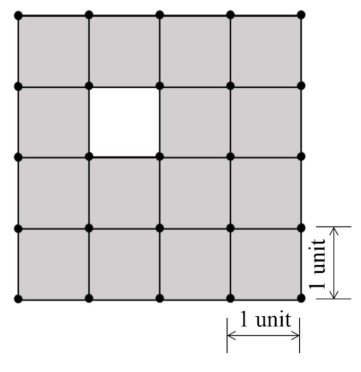
\includegraphics[scale=0.5]{q4}
            \label{fig:q4}
         \end{figure}[H]

         What is the maximum number of squares without a 'hole in the interior' that can be formed within the $4 \times 4$ grid using the unit squares as building blocks?
         \begin{enumerate}
            \begin{multicols}{4}
               \item 15
               \item 20
               \item 21
               \item 26
            \end{multicols}
         \end{enumerate}

   \item An art gallery engages a security guard to ensure that the items displayed are protected. The diagram below represents the plan of the gallery where the boundary walls are opaque. The location the security guard posted is identified such that all the inner space (shaded region in the plan) of the gallery is within the line of sight of the security guard.

         If the security guard does not move around the posted location and has a $360^\circ$ view, which one of the following correctly represents the set of ALL possible locations among the locations P, Q, R and S, where the security guard can be posted to watch over the entire inner space of the gallery.

         \begin{figure}[H]
            \centering
            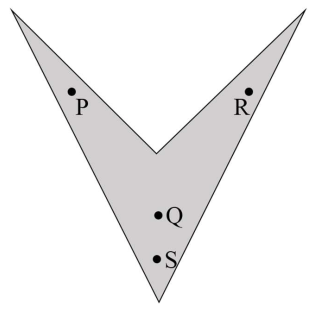
\includegraphics[scale=0.7]{q5}
            \label{fig:q5}
         \end{figure}

         \begin{enumerate}
            \item P and Q
            \item Q
            \item Q and S
            \item R and S
         \end{enumerate}
\end{enumerate}
\normalsize\textbf{Q1 - Q5 carry one mark each.}

\begin{enumerate}
   \setcounter{enumi}{5}
   \item Mosquitoes pose a threat to human health. Controlling mosquitoes using chemicals may have undesired consequences. In Florida, authorities have used genetically modified mosquitoes to control the overall mosquito population. It remains to be seen if this novel approach has unforeseen consequences.

         Which one of the following is the correct logical inference based on the information in the above passage?
         \begin{enumerate}
            \item Using chemicals to kill mosquitoes is better than using genetically modified mosquitoes because genetic engineering is dangerous
            \item Using genetically modified mosquitoes is better than using chemicals to kill mosquitoes because they do not have any side effects
            \item Both using genetically modified mosquitoes and chemicals have undesired consequences and can be dangerous
            \item Using chemicals to kill mosquitoes may have undesired consequences but it is not clear if using genetically modified mosquitoes has any negative consequence
         \end{enumerate}

   \item Consider the following inequalities.
         \begin{align}
            2x - 1 > 7 \\
            2x - 9 < 1
         \end{align}
         Which one of the following expressions below satisfies the above two inequalities?
         \begin{enumerate}
            \item $x \leq -4$
            \item $-4 < x \leq 4$
            \item $4 < x < 5$
            \item $x \geq 5$
         \end{enumerate}

   \item Four points P$(0, 1)$, Q$(0, -3)$, R$(-2, -1)$, and S$(2, -1)$ represent the vertices of a quadrilateral.\\
         What is the area enclosed by the quadrilateral?
         \begin{enumerate}
            \begin{multicols}{4}
               \item 4
               \item $4\sqrt{2}$
               \item 8
               \item $8\sqrt{2}$
            \end{multicols}
         \end{enumerate}

   \item In a class of five students P, Q, R, S and T, only one student is known to have copied in the exam. The disciplinary committee has investigated the situation and recorded the statements from the students as given below.

         \begin{itemize}
            \item \textbf{Statement of P}: R has copied in the exam.
            \item \textbf{Statement of Q}: S has copied in the exam.
            \item \textbf{Statement of R}: P did not copy in the exam.
            \item \textbf{Statement of S}: Only one of us is telling the truth.
            \item \textbf{Statement of T}: R is telling the truth.
         \end{itemize}

         The investigating team had authentic information that S never lies.

         Based on the information given above, the person who has copied in the exam is
         \begin{enumerate}
            \begin{multicols}{4}
               \item R
               \item P
               \item Q
               \item T
            \end{multicols}
         \end{enumerate}

   \item Consider the following square with the four corners and the center marked as P, Q, R, S and T respectively.

         Let X, Y and Z represent the following operations:

         X: rotation of the square by 180 degree with respect to the S-Q axis.

         Y: rotation of the square by 180 degree with respect to the P-R axis.

         Z: rotation of the square by 90 degree clockwise with respect to the axis perpendicular, going into the screen and passing through the point T.

         Consider the following three distinct sequences of operation (which are applied in the left to right order).

         \begin{enumerate}
            \item XYZZ
            \item XY
            \item ZZZZ
         \end{enumerate}

         Which one of the following statements is correct as per the information provided above?

         \begin{figure}[H]
            \centering
            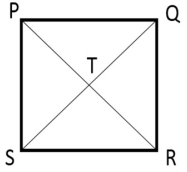
\includegraphics[scale=0.5]{q10}
            \label{fig:q10}
         \end{figure}
         \begin{enumerate}
            \item The sequence of operations (1) and (2) are equivalent
            \item The sequence of operations (1) and (3) are equivalent
            \item The sequence of operations (2) and (3) are equivalent
            \item The sequence of operations (1), (2) and (3) are equivalent
         \end{enumerate}
\end{enumerate}

\normalsize\textbf{Q11 - Q35 carry one mark each.}

\begin{enumerate}
   \setcounter{enumi}{10}
   \item A student reported following arsenic concentrations in water samples:

         \begin{table}
            \begin{center}
               \begin{tabular}{|c|c|c|c|c|c|c|c|c|}
                  \hline
                  Arsenic concentration (mg/L) & 0.10 & 0.12 & 0.20 & 0.05 & 0.40 & 0.30 & 0.35 \\
                  \hline
               \end{tabular}
            \end{center}
            \label{tab:q11}
         \end{table}

         Which one of the following is a correct statement about arsenic concentration distribution?
         \begin{enumerate}
            \item Arsenic concentration distribution is symmetric
            \item Arsenic concentration distribution is positively skewed
            \item Arsenic concentration distribution is negatively skewed
            \item Arsenic concentration is following Weibull distribution
         \end{enumerate}

   \item X is normally distributed with following data (25.8, 36.6, 26.3, 21.8, 27.2). Select the correct statement about X ($t_{\text{crit},\,\alpha=0.05,4}=2.132$):

         \begin{enumerate}
            \item Population mean $\leq 25$ with 95\% confidence
            \item Population mean $\leq 25$ with 100\% confidence
            \item Population mean $> 25$ with 95\% confidence
            \item Population mean $> 25$ with 100\% confidence
         \end{enumerate}

   \item Assuming $s > 0$; Laplace transform for $f(x) = \sin(ax)$ is
         \begin{enumerate}
            \item $\frac{a}{s^2 + a^2}$
            \item $\frac{s}{s^2 + a^2}$
            \item $\frac{a}{s^2 - a^2}$
            \item $\frac{s}{s^2 - a^2}$
         \end{enumerate}

   \item Given $\vec{P}$ is $m \times n$ matrix, $\vec{Q}$ is $n \times l$ matrix, $\vec{R}$ and $\vec{S}$ are $n \times n$ matrices, and superscript T denotes transpose. Consider

         \begin{quote}
            Relationship 1: $(\vec{PQ})^T = \vec{Q}^T\vec{P}^T$

            Relationship 2: $(\vec{RS})^{-1} = \vec{S}^{-1}\vec{R}^{-1}$
         \end{quote}

         Which one of the following is correct?
         \begin{enumerate}
            \item Relationship 1 is false; Relationship 2 is false
            \item Relationship 1 is true; Relationship 2 is false
            \item Relationship 1 is true; Relationship 2 is true
            \item Relationship 1 is false; Relationship 2 is true
         \end{enumerate}

   \item Specific conductance is used in water analysis to indirectly estimate dissolved solids. The measurements used in the method accounts for
         \begin{enumerate}
            \begin{multicols}{4}
               \item Cations only
               \item All ions
               \item Anions only
               \item Un-ionized species
            \end{multicols}
         \end{enumerate}

   \item Ten litres of the sample was filtered through a membrane filter and the filter was transferred to solid agar media which supports growth of coliform organisms. After incubation at 37 $^\circ$C for 48 hours, the agar plates showed an average of 64 colonies per plate. What was the average concentration of coliform organisms (in \textbf{C}olony \textbf{F}orming \textbf{U}nits per unit volume) in the original water sample?
         \begin{enumerate}
            \begin{multicols}{2}
               \item 64 CFU/ml
               \item 640 CFU/ml
               \item $6.4 \times 10^{-3}$ CFU/ml
               \item $64 \times 10^{-3}$ CFU/ml
            \end{multicols}
         \end{enumerate}

   \item Reverse Transcriptase Polymerase Chain Reaction is an analytical procedure used in detection of pathogenic microorganisms. Which one of the following statements is NOT correct in this context?
         \begin{enumerate}
            \item It is used for identifying presence or absence of specific RNA in samples.
            \item It is used only for identifying Corona Viruses, including SARS CoV2 in samples.
            \item It cannot differentiate between viable and inactivated viruses.
            \item It is based on conversion of RNA to DNA followed by DNA amplification.
         \end{enumerate}

   \item Consider the following statements

         Statement 1: Goodrich method for reservoir routing is based on hydrologic flood routing method.

         Statement 2: Muskingum method for channel routing is based on hydraulic flood routing method.

         Which one of the following is correct?
         \begin{enumerate}
            \item Statement 1 is false; Statement 2 is false
            \item Statement 1 is true; Statement 2 is false
            \item Statement 1 is true; Statement 2 is true
            \item Statement 1 is false; Statement 2 is true
         \end{enumerate}

   \item The correct order of hydraulic conductivity for the geologic formations is
         \begin{enumerate}
            \item Aquifer $>$ Aquitard $>$ Aquiclude $>$ Aquifuge
            \item Aquifer $<$ Aquitard $<$ Aquiclude $<$ Aquifuge
            \item Aquitard $>$ Aquifer $>$ Aquifuge $>$ Aquiclude
            \item Aquifer $>$ Aquiclude $>$ Aquitard $>$ Aquifuge
         \end{enumerate}

   \item Centrifugal pumps with suction pipe (shown by solid arrow) and delivery pipe (shown by dotted arrow) are shown in the figures. Choose the option that gives the correct connection
         \begin{enumerate}
            \item 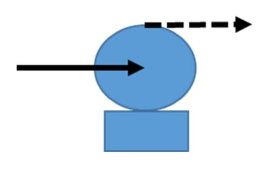
\includegraphics[scale=0.4]{o20a}
            \item 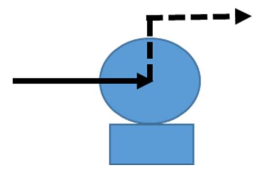
\includegraphics[scale=0.4]{o20b}
            \item 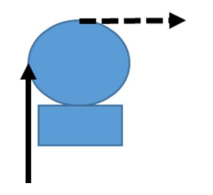
\includegraphics[scale=0.4]{o20c}
            \item 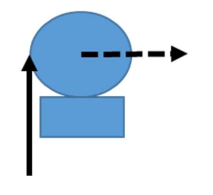
\includegraphics[scale=0.4]{o20d}
         \end{enumerate}

   \item Carbon dioxide is used in recarbonation process. A solution has 1 mole/L supersaturated calcium carbonate. Estimated amount of carbon dioxide (in grams) needed to completely convert calcium carbonate to calcium ions in 1 litre solution is
         \begin{enumerate}
            \item 44.000 gram
            \item 0.044 gram
            \item 40.000 gram
            \item 0.040 gram
         \end{enumerate}

   \item A river water sample has pH of 4 and suspended solids concentration of 100 mg/L. If, alum is chosen as a coagulant, what will be the coagulation mechanism?
         \begin{enumerate}
            \item Ionic layer compression only
            \item Sweep coagulation and Polymer bridging
            \item Polymer bridging only
            \item Charge neutralization, surface adsorption, ionic layer compression
         \end{enumerate}

   \item Which one of the following is most commonly used raw material in flue gas desulfurization units?
         \begin{enumerate}
            \item Limestone
            \item Titanium Oxide
            \item Fenton reagent
            \item Beryllium Oxide
         \end{enumerate}

   \item Leachate generated from a legacy municipal solid waste dumping site has to be collected and managed carefully. Which one of the following statements is correct in the context of treatment of leachate from such a site?
         \begin{enumerate}
            \item Settling chamber followed by micro-filtration units are required.
            \item Modular treatment units targeting dissolved organic matter and salts are required.
            \item Only biological treatment units like ASP with extended aeration are required.
            \item Only a combination of anaerobic-aerobic treatment units is required.
         \end{enumerate}

   \item Which one of the following statements is correct regarding Global warming?
         \begin{enumerate}
            \item Water vapour does not contribute to global warming.
            \item Global warming is likely to increase the productivity of plants due to CO$_2$ fertilization.
            \item CFCs do not cause global warming, but can cause ozone layer depletion in stratosphere.
            \item HFCs and HCFCs are good substitutes for the ozone depleting substances as they cause neither global warming nor ozone layer depletion.
         \end{enumerate}

   \item In context of ecosystems, which one of the following is NOT a correct statement?
         \begin{enumerate}
            \item The growth of an organism such as a plant may be dependent on a number of different factors such as sunlight, mineral nutrients (nitrates, phosphates, etc.), etc. Liebig's law states that, growth occurs at the rate permitted by the most limiting factor.
            \item The carrying capacity of a population is determined by its limiting resources. Carrying capacity is the upper limit of an ecosystem up to which it can provide the basic needs to the population under given circumstances.
            \item The Ramsar convention on lakes and backwater systems of International importance is an international treaty for the conservation and sustainable use of lakes and backwater systems. The treaty was signed in 1981 and became effective in 1985.
            \item A Red Data Book contains lists of species whose continued existence is threatened. Species are classified into different categories of perceived risk. Each Red Data Book usually deals with a specific group of animals or plants and fungi.
         \end{enumerate}

   \item Which one of the following statements correctly defines the concept of 'Extended Producer's Responsibility'?
         \begin{enumerate}
            \item The responsibility of a producer for environmentally sound disposal of the product after the end of its life
            \item The responsibility of a producer for environmentally sound manufacturing process for the product
            \item The responsibility of a producer for environmentally sound management of the product from manufacturing stage until it is sold in the market
            \item The responsibility of a producer for environmentally sound management of the product until the end of its life
         \end{enumerate}
\end{enumerate}

\textbf{MSQ}

\begin{enumerate}
   \setcounter{enumi}{27}
   \item If G represents Gibbs free energy, select the correct statement(s)
         \begin{enumerate}
            \item If $\Delta G = 0$, reaction will proceed only in one direction
            \item If $\Delta G = 0$, reaction will be in equilibrium
            \item If $\Delta G < 0$, reaction will proceed forward
            \item If $\Delta G > 0$, reaction will not proceed forward
         \end{enumerate}

   \item For effluents generated by a molasses based distillery and wood based pulp and paper industry, which of the following statement(s) is/are NOT correct?
         \begin{enumerate}
            \item Both the effluents have dark colour.
            \item Both the effluents have high toxicity.
            \item Both the effluents generally have BOD greater than 15,000 ppm.
            \item Both the effluents have high pH.
         \end{enumerate}

   \item PM$_{2.5}$ concentrations in ambient air can be measured using
         \begin{enumerate}
            \item Beta attenuation method
            \item Chemiluminescence method
            \item Gravimetric method
            \item Non dispersive infrared spectroscopy method
         \end{enumerate}

   \item Biodegradable wastes like vegetable peelings from kitchen are usually processed by composting techniques. Which of the following option(s) regarding the processing of biodegradable wastes is/are correct?
         \begin{enumerate}
            \item Vermi-composting is relatively faster than windrow composting, however vermi-composting is not frequently used on large commercial scale.
            \item The windrow height should be as short as possible as large windrow height may cause compaction due to the self-weight.
            \item The windrow height should be as large as possible as that will help to ensure appropriate temperature within the windrow.
            \item Earthworms facilitate the growth of microorganisms and break down complex organic molecules to simpler ones using enzymatic secretions.
         \end{enumerate}

   \item As per `Hazardous and Other Wastes' (Management and Transboundary Movement) Rules, 2016 of Govt. of India, the import of hazardous and other wastes from any country shall NOT be permitted for which of the following option(s)?
         \begin{enumerate}
            \item Recovery, reuse and recycle
            \item Disposal in abandoned mines
            \item Safe disposal in engineered landfills
            \item Utilization, including co-processing
         \end{enumerate}

   \item The Ministry of Environment, Forest and Climate Change (MoEF\&CC), Govt. of India has published the Environment Impact Assessment (EIA) draft Notification 2020, intended to replace the existing EIA Notification, 2006 under the Environment (Protection) Act, 1986. Which of the following is/are the key change(s) from existing regulation?
         \begin{enumerate}
            \item Removal of several project/ activities from the purview of public consultation.
            \item A list of projects has been included under Category B2, expressly exempted from the requirement of an EIA.
            \item All the project related activities are brought under the purview of necessary public consultation.
            \item A list of projects has been included under Category B2, bringing them under the requirement of detailed EIA.
         \end{enumerate}

   \item $\displaystyle \lim_{x \to 0} \frac{\sqrt{1+x} - 1}{x}$ is \underline{\hspace{2cm}} \textit{(rounded off to one decimal place)}

   \item The following figure shows a 2-hour unit hydrograph (1 cm rainfall excess) for a catchment area of 540 hectare.

         \begin{figure}[H]
            \centering
            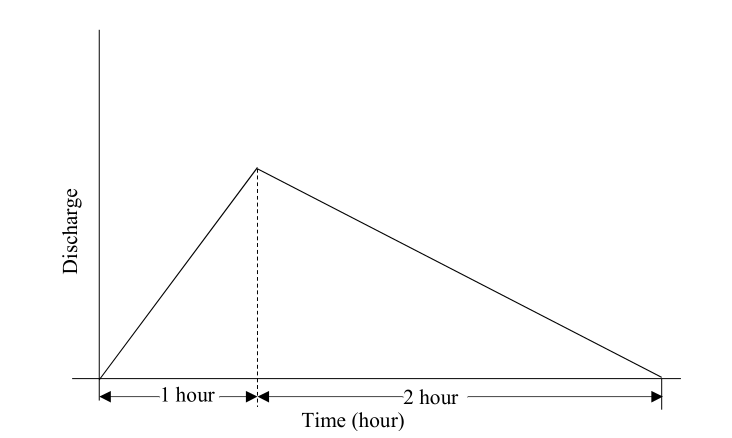
\includegraphics[scale=0.6]{q35}
            \label{fig:q35}
         \end{figure}

         The peak discharge (in m$^3$/s, \textit{rounded off to one decimal place}) of the above unit hydrograph is \underline{\hspace{2cm}}
\end{enumerate}

\normalsize\textbf{Q36 - Q65 carry two marks each.}

\begin{enumerate}
   \setcounter{enumi}{35}
   \item Given, $y = f(x)$; $\frac{d^2y}{dx^2} + 4y = 0$; $y(0) = 0$; $\frac{dy}{dx}(0) = 1$. The problem is a/an
         \begin{enumerate}
            \item initial value problem having solution $y = x$
            \item boundary value problem having solution $y = x$
            \item initial value problem having solution $y = \frac{1}{2} \sin 2x$
            \item boundary value problem having solution $y = \frac{1}{2} \sin 2x$
         \end{enumerate}

   \item Eigen values of the matrix $\myvec{ 0 & 1 \\ -2 & 3}$ are
         \begin{enumerate}
            \item 1 and 2
            \item 1 and 3
            \item 1 and $-2$
            \item 0 and 3
         \end{enumerate}

   \item For an exponentially growing microbial culture, the specific growth rate ($\mu$) is related to its doubling time ($t_d$) by which one of the following relations?
         \begin{enumerate}
            \item $t_d = \mu$
            \item $t_d = \mu^2$
            \item $t_d = \frac{1}{\mu} \ln 2$
            \item $t_d = \frac{1}{2} \ln \mu$
         \end{enumerate}

   \item A microbial culture, with a specific growth rate of $\mu_1$ (per hour), is being grown in a continuous reactor at steady state with hydraulic retention time (HRT) of 24 hours. This reactor is subjected to a perturbation by reducing the HRT to 12 hours. The reactor recovers from the perturbation and comes to a new steady state with a new specific growth rate of $\mu_2$ (per hour). Which one of the following statements is correct?
         \begin{enumerate}
            \item $\mu_1 = \mu_2$
            \item $\mu_1 = 0.5\,\mu_2$
            \item $\mu_2 = 0.5\,\mu_1$
            \item $\mu_2 = e^{0.5}\,\mu_1$
         \end{enumerate}

   \item Which one of the following statements is NOT correct with respect to a batch reactor?
         \begin{enumerate}
            \item No reactant is added after the reactor has started operation.
            \item No product is withdrawn during the course of the reactor operation.
            \item The reactor operates under steady state.
            \item The reactor operation is carried out for a pre-specified duration.
         \end{enumerate}

   \item A bag filter is used for removal of particulate matter having a range of sizes. The correct sequence of air filtration mechanisms for their removal, in order of decreasing size, is
         \begin{enumerate}
            \item Diffusion, Impaction, Disintegration
            \item Disintegration, Impaction, Interception
            \item Diffusion, Impaction, Interception
            \item Impaction, Interception, Diffusion
         \end{enumerate}

   \item A relatively calm room has background sound power level (SPL) of 30 decibels (dB). A television and a radio with SPL of 80 dB and 70 dB, respectively, started operating simultaneously in this room. Given the reference sound power is $10^{-12}$ Watts, what will be the resulting SPL in the room, assuming all the sources operate independently?
         \begin{enumerate}
            \item 180.0 dB
            \item 80.4 dB
            \item 82.4 dB
            \item 150.0 dB
         \end{enumerate}
\end{enumerate}
\textbf{MSQ}
\begin{enumerate}
   \setcounter{enumi}{42}
   \item During night, in troposphere, which of the following is/are NOT correct
         \begin{enumerate}
            \item NO$_2$ + h$\nu$ $\rightarrow$ NO + O
            \item Most of the NOx (i.e., NO + NO$_2$) converts to NO
            \item NO + O$_3$ $\rightarrow$ NO$_2$ + O$_2$
            \item Most of the NOx (i.e., NO + NO$_2$) converts to NO$_2$
         \end{enumerate}

   \item A typical plasmid-free bacterial cell having a single chromosome consists of $\sim$55\% protein, $\sim$3\% DNA and $\sim$21\% RNA, where '\%' represents percentage of dry weight. Assuming there are 2500 different types of protein molecules (with at least one copy number) being expressed in a living bacterial cell at any given time, which of the following statement(s) is/are NOT correct with respect to the number of intracellular DNA, RNA and protein molecules?
         \begin{enumerate}
            \item DNA = RNA = Protein $\geq$ 2500
            \item DNA = RNA = 1; Protein $\geq$ 2500
            \item DNA = 1; RNA = Protein $\geq$ 2500
            \item DNA = 1; RNA $>$ Protein $\geq$ 2500
         \end{enumerate}

   \item Average values of the re-aeration rate constant for river X and river Y are 0.92 per day and 1.12 per day, respectively. Average de-oxygenation rate constants for the same rivers are 0.23 per day and 0.35 per day respectively. Then, which of the following statement(s) is/are correct?
         \begin{enumerate}
            \item Self-purification capacity of river Y is more than that of river X.
            \item Self-purification capacity of river X is more than that of river Y.
            \item River Y has higher turbulence and/or higher velocity and/or higher algal growth compared to river X.
            \item Pollutants in river X are more biodegradable than that in river Y.
         \end{enumerate}

   \item Which of the following statement(s) is/are NOT correct while comparing continuously stirred tank reactor (CSTR) and plug flow reactor (PFR)?
         \begin{enumerate}
            \item CSTR and PFR are normally operated under steady state condition.
            \item There is complete homogeneity in the CSTR while there are concentration variations within the PFR.
            \item The overall reaction carried out in a PFR is always higher than that in a CSTR for same total volume.
            \item Reaction kinetics do not play any role in choosing between a CSTR and PFR.
         \end{enumerate}

   \item According to the National Ambient Air Quality Standards (Central Pollution Control Board, Govt. of India, notification 2009) which of the following statement(s) is/are correct?
         \begin{enumerate}
            \item SO$_2$ and NO$_2$ have annual average standards; while O$_3$ and CO have eight hour average standards.
            \item SO$_2$ and CO have annual average standards; while O$_3$ and NO$_2$ have eight hour average standards.
            \item SO$_2$ and CO have eight hour average standards; while O$_3$ and NO$_2$ have hourly average standards.
            \item SO$_2$ and NO$_2$ have 24 hour average standards; while O$_3$ and CO have hourly average standards.
         \end{enumerate}

   \item Consider the figure shown below for three different cases:

         \begin{figure}[H]
            \centering
            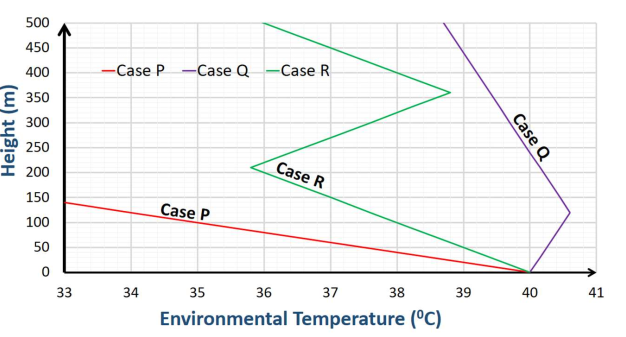
\includegraphics[scale=0.6]{q48}
            \label{fig:q48}
         \end{figure}

         Which of the following statement(s) is/are correct for surface level emissions, given the environmental temperature?

         \begin{enumerate}
            \item Case P represents unstable atmosphere and results in higher dispersion of emissions.
            \item Case Q represents subsidence inversion and results in higher dispersion of emissions than Case P.
            \item Case Q represents elevated inversion and results in lower dispersion of emissions than Case P.
            \item Case R represents subsidence inversion and results in lower dispersion of emissions than Case P.
         \end{enumerate}

   \item As per the Solid Waste Management Rules of 2016 (Govt. of India), which of the following statement(s) is/are correct?
         \begin{enumerate}
            \item Biodegradable wastes should be processed biologically preferably in decentralized facilities at the sources of generation.
            \item Biodegradable wastes should be processed biologically preferably in centralized facilities away from the sources of generation.
            \item Used sanitary pads and napkins should be wrapped and disposed into the domestic hazardous waste containers.
            \item Non-biodegradable components with a heat content more than 1500 kcal/kg should be used for power generation or Refuse Derived Fuel (RDF) manufacture.
         \end{enumerate}

   \item Carbon cycle, nitrogen cycle and phosphorus cycle play important role in the ecosystems. Which of the following statement(s) is/are NOT correct about the phosphorus cycle?
         \begin{enumerate}
            \item Shortage of phosphorus can be a limiting factor in many ecosystems, however, its excess can stimulate eutrophication.
            \item Organic phosphates exist in various rock and soil minerals.
            \item Like carbon cycle, phosphorus also has a gaseous phase and can move into far away ecosystems.
            \item Human interventions like application of phosphorus fertilizers cause much phosphorus to get into the ocean.
         \end{enumerate}

   \item Which of the following statement(s) is/are correct regarding National Green Tribunal (NGT) of India?
         \begin{enumerate}
            \item NGT Act 2010 draws inspiration from the India's constitutional provision of Article 21 - Protection of life and personal liberty, which assures the citizens of India the right to a healthy environment.
            \item A retired Judge of the Supreme Court, can be the Chairperson of the NGT.
            \item NGT Act 2017 is based on the India's constitutional provision of Article 361 - Protection of Biodiversity and Environmental Protection, which bestows the citizens of India with a duty to protect all abiotic and biotic components of the environment.
            \item The NGT is mandated to make and endeavor for disposal of applications or appeals finally within 45 days of filing of the same.
         \end{enumerate}

   \item The area of the region (\textit{rounded off to one decimal place}) enclosed between the curves $y = x$ and $y = 3\sqrt{x}$ and between the lines $x = 0$ and $x = 1$ is \underline{\hspace{2cm}} units.

   \item An individual has four different email accounts. 60\% of emails come into his corporate account, 30\% come into his gmail account and remaining 10\% are equally divided into his yahoo and zoho accounts. Only 1\% of the emails in his corporate accounts are spam, whereas corresponding percentages for gmail, yahoo and zoho accounts are 2\%, 3\% and 3\%, respectively. Assuming that the same spam filter is used in all the four email accounts, the probability (in percentage, \textit{rounded off to one decimal place}) of having a randomly selected email as spam is \underline{\hspace{2cm}}.

   \item A solution has 0.001 mole/L zinc ions having pH of 6. Solubility product of zinc hydroxide is given as $8 \times 10^{-18}$ (mole/L)$^3$. Ignoring activity corrections, the ratio (\textit{rounded off to two decimal places}) of reaction coefficient to solubility product would be \underline{\hspace{2cm}}.

   \item The Henry's law constant of CO$_2$ is $3.4 \times 10^{-2}$ M per atm in neutral water at 25$^\circ$C. The dissolved CO$_2$ (i.e., CO$_2$.H$_2$O) at equilibrium undergoes the following reactions.

         \begin{align*}
            \text{CO}_2 \cdot \text{H}_2\text{O} & \rightleftharpoons \text{H}^+ + \text{HCO}_3^- \quad \text{(Equilibrium constant = $4.3 \times 10^{-7}$ M)}    \\
            \text{HCO}_3^-                       & \rightleftharpoons \text{H}^+ + \text{CO}_3^{2-} \quad \text{(Equilibrium constant = $4.7 \times 10^{-11}$ M)}
         \end{align*}

         If ambient CO$_2$ concentration is 300 ppm, the total dissolved CO$_2$ (in $\mu$M, \textit{rounded off to one decimal place}) is \underline{\hspace{2cm}}.

   \item An isolated storm of 3 hours occurred over a catchment area in the following manner:

         \begin{table}[H]
            \centering
            \begin{tabular}{|c|c|c|c|c|}
               \hline
               \multirow{2}{*}{\% Catchment Area} & \multirow{2}{*}{$\phi$-index (cm/hour)} & \multicolumn{3}{|c|}{Rainfall (cm)}                                           \\\cline{3-5}
                                                  &                                         & 1$^\text{st}$ hour                  & 2$^\text{nd}$ hour & 3$^\text{rd}$ hour \\
               \hline
               15                                 & 0.5                                     & 0.4                                 & 2.5                & 1.6                \\\hline
               35                                 & 1.0                                     & 0.8                                 & 3.0                & 2.1                \\\hline
               50                                 & 0.8                                     & 0.6                                 & 2.6                & 1.9                \\\hline
            \end{tabular}
            \label{tab:q56}
         \end{table}

         Total rainfall excess (in cm, \textit{rounded off to one decimal place}) over the catchment for the above storm is \underline{\hspace{2cm}}.

   \item Two reservoirs having a difference of 20 m in their water surface elevations are connected through a confined aquifer (thickness = 5 m, length = 2 km, hydraulic conductivity $K = 3 \times 10^{-3}$ m/s, and porosity $\eta = 0.3$) as shown in the following figure (drawn not to scale).

         \begin{figure}[H]
            \centering
            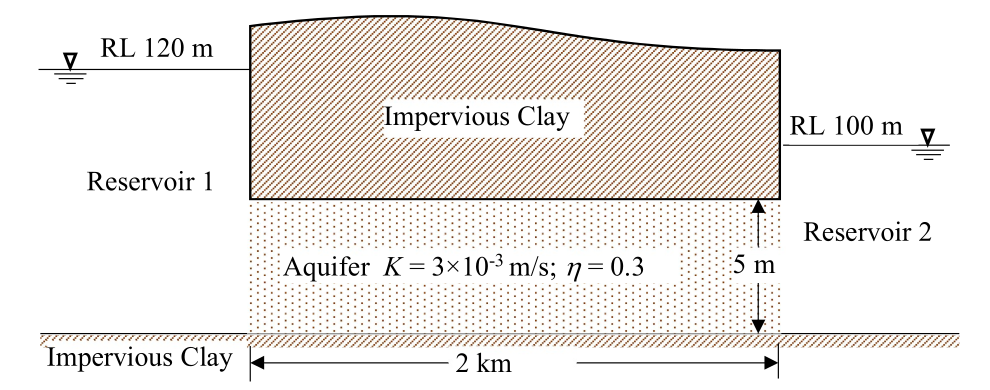
\includegraphics[scale=0.4]{q57}
            \label{fig:q57}
         \end{figure}

         If the Reservoir 1 is contaminated by a pollutant then the time (in days, \textit{rounded off to one decimal place}) taken by the pollutant to reach to the Reservoir 2 under advection will be \underline{\hspace{2cm}}.

   \item A venturimeter along with a differential manometer was installed to measure flow in a water pipeline as shown in the following figure (not drawn to scale).

         \begin{figure}[H]
            \centering
            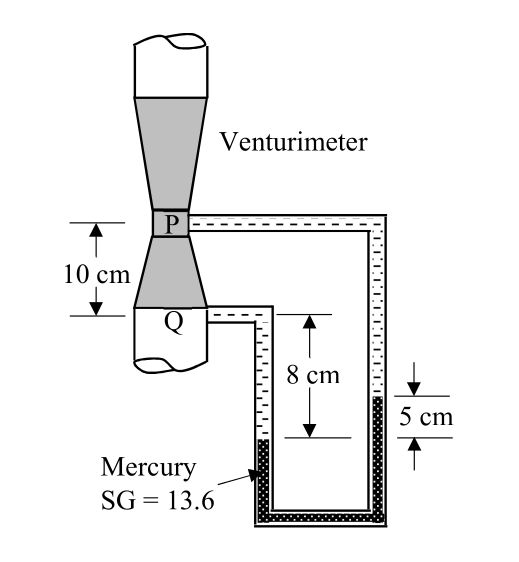
\includegraphics[scale=0.5]{q58}
            \label{fig:q58}
         \end{figure}

         Taking specific weight of water as 9810 N/m$^3$, the pressure difference (in Pa, \textit{rounded off to one decimal place}) between point Q and P is \underline{\hspace{2cm}}.

   \item Two reservoirs having a difference of 10 m in their water surface elevations are connected by a pipeline (diameter = 10 cm, length = 50 m, and friction factor $f = 0.02$). If the last 25 m length of the pipeline is replaced by a same material pipe of diameter 20 cm then neglecting minor losses the discharge (in \%, \textit{rounded off to one decimal place}) will increase by \underline{\hspace{2cm}}.

   \item The depth of flow (in m, \textit{rounded off to two decimal places}) in a hydraulically efficient rectangular channel ($n = 1/80$) to carry a discharge of 64 m$^3$/s at bed slope 0.01 is \underline{\hspace{2cm}}.

   \item Clean water is passed through a bed of uniform spherical sand at a filtration velocity of 0.002 m/sec. The sand grains are 0.4 mm in diameter and have a specific gravity of 2.65. Bed depth is 0.67 m and porosity ($\eta$) is 0.35. Given, water density = 998.2 kg/m$^3$; water dynamic viscosity = $1.002 \times 10^{-3}$ Pa.s. Friction factor ($f$) is given as: $f = 1.75 + \{150 \times (1-\eta)/(Re)\}$ where $Re$ is Reynolds number. The headloss (in m, \textit{rounded off to three decimal places}) calculated using the Carmen-Kozney equation is \underline{\hspace{2cm}}.

   \item A sewage treatment plant with a capacity of 10 million litres per day (MLD) is treating the sewage through an aerobic biological process. The inlet and outlet BOD are measured as 100 and 30 mg/l, respectively. If the mixed microbial culture has an observed biomass yield of 0.5 g Volatile Suspended Solids (VSS)/g BOD, the sludge production rate (in kg per day, \textit{rounded off to one decimal place}) when the plant is operating at 80\% capacity will be \underline{\hspace{2cm}}.

   \item A centrifuge is processing 1000 litres per hour of water containing 2 g per litre of suspended solids. The thickened slurry coming out of the centrifuge has solids concentration of 20 g per 100 ml. If the centrifuge has 99\% efficiency based on solids separation, the flow rate (in litres per hour, \textit{rounded off to one decimal place}) of the supernatant stream will be \underline{\hspace{2cm}}.

   \item A ground level source emits 1000 g per day of SO$_2$. In vicinity of the source, ambient temperature is measured at 10 m and 110 m as 25$^\circ$C and 24.5$^\circ$C, respectively. The mean wind speed is found to be 2 m per second. The dispersion coefficients at 1000 m downwind distance from the source are given in table below:

   \begin{table}[H]
      \centering
      \begin{tabular}{|c|c|c|c|}
         \hline
         \multirow{2}{*}{} & \multicolumn{3}{c|}{Dispersion coefficients (in m)} \\
         \cline{2-4}
         & Stable & Neutral & Unstable \\\hline
         Crosswind direction & 50.5 & 80.0 & 156.0 \\\hline
         Vertical direction  & 21.4 & 41.5 & 110.2 \\\hline
      \end{tabular}
      \label{tab:dispersion}
   \end{table}

   Estimated ground level concentration (in $\mu$g/m$^3$, \textit{rounded off to two decimal places}) of SO$_2$ at a downwind distance of 1000 m (at the plume centerline) from the source is \underline{\hspace{2cm}}.

   \item Figure below gives the heat inflow into the furnace of a waste-to-energy plant along with the heat outflows from the furnace.

   \begin{figure}[H]
      \centering
      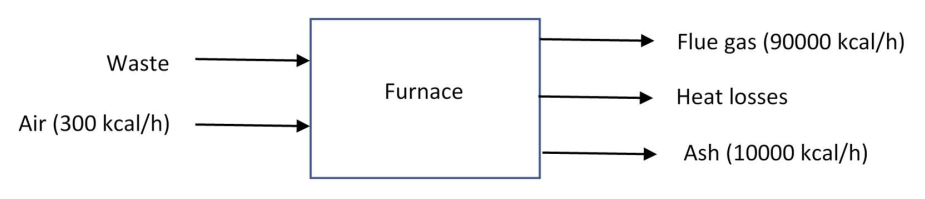
\includegraphics[scale=0.4]{q65}
      \label{fig:q65}
   \end{figure}

   Assume: (i) total heat loss equal to 3\% of heat released while burning waste, (ii) sensible heat of the waste is negligible, (iii) complete burning of the waste is ensured. If the waste feed rate into this plant is 70 kg/h, the heat content of the waste (in kcal/kg, \textit{rounded off to one decimal place}) is \underline{\hspace{2cm}}.
\end{enumerate}
\end{document}